\documentclass[12pt]{article}
\usepackage[english]{babel}
\usepackage[utf8]{inputenc}

\usepackage{geometry}
\geometry{
	letterpaper, 
	portrait, 
	top=.75in,
	left=.8in,
	right=.75in,
	bottom=.5in		} 	% Page Margins
	
%% additional packages for nice things
\usepackage{amsmath} 	% for most math
\usepackage{commath} 	% for abs
\usepackage{lastpage}	% for page count
\usepackage{amssymb} 	% for therefore
\usepackage{graphicx} 	% for image handling
\usepackage{wrapfig} 	% wrap figures
\usepackage[none]{hyphenat} % for no hyphenations
\usepackage{booktabs} 	% enhanced table qualities
\usepackage{array} 		% for >{} column characterisctis
\usepackage{physics} 	% for easier derivative \dv....
\usepackage{tikz} 		% for graphic@!
\usepackage{circuitikz} % for circuits!
\usetikzlibrary{arrows.meta} % for loads
\usepackage[thicklines]{cancel}	% for cancels
\usepackage{xcolor}		% for color cancels
\usepackage[per-mode=fraction]{siunitx} % for si units and num
\usepackage{fancyhdr} 	% for header
\usepackage{comment}	% for ability to comment out large sections
\usepackage{multicol}	% for multiple columns using multicols
\usepackage[framed,numbered]{matlab-prettifier} % matlab sytle listing
\usepackage{marvosym} 	% for boltsymbol lightning
\usepackage{pdflscape} 	% for various landscape pages in portrait docs.
\usepackage{float}
\usepackage{fancyvrb}	% for Verbatim (a tab respecting verbatim)
\usepackage{enumitem}	% for [resume] functionality of enumerate

%% package config 
\sisetup{output-exponent-marker=\ensuremath{\mathrm{E}}} % for engineer E
\renewcommand{\CancelColor}{\color{red}}	% for color cancels
\lstset{aboveskip=2pt,belowskip=2pt} % for more compact table
\def\arraystretch{1.4} % adjust size of arrays
%\arraycolsep=1.4pt\def
\setlength{\parindent}{0cm} % Remove indentation from paragraphs
\setlength{\columnsep}{0.5cm}
\lstset{
	style      = Matlab-editor,
	basicstyle = \ttfamily\footnotesize, % if you want to use Courier - not really used?
}
\renewcommand*{\pd}[3][]{\ensuremath{\dfrac{\partial^{#1} #2}{\partial #3}}} % for larger pd fracs
\renewcommand{\real}[1]{\mathbb{R}\left\{ #1 \right\}}	% for REAL symbol
\newcommand{\imag}[1]{\mathbb{I}\left\{ #1 \right\}}	% for IMAG symbol
\definecolor{m}{rgb}{1,0,1}	% for MATLAB matching magenta
	
%% custom macros
\newcommand\numberthis{\addtocounter{equation}{1}\tag{\theequation}} % for simple \numberthis command
\newcommand{\equal}{=} % so circuitikz can have an = in the labels
\newcolumntype{L}[1]{>{\raggedright\let\newline\\\arraybackslash\hspace{0pt}}m{#1}}
\newcolumntype{C}[1]{>{\centering\let\newline\\\arraybackslash\hspace{0pt}}m{#1}}
\newcolumntype{R}[1]{>{\raggedleft\let\newline\\\arraybackslash\hspace{0pt}}m{#1}}

%% Header
\pagestyle{fancy} % for header stuffs
\fancyhf{}
\rhead{Thad Haines \\ Page \thepage\ of \pageref{LastPage}}
\chead{Talking Points \\ Week of January 21, 2019}
\lhead{Research \\ }
% spacing
\headheight 29 pt
\headsep 6 pt

\begin{document}
	\paragraph{Recent Progress:}
	\begin{enumerate}
		\item Simulation data output as \verb|.mat| achieved.
		
		\item Verification of Frequency response begun.
		\subitem Initial 'EE554.sav' 3 Bus load step result plots on page 2.
		
		\item Added custom model parsing ability to dyd parser
		\subitem Any line starting with \verb|#!| in a dyd file will correspond to LTD model parameters.
		
		\item GitHub repository updated:
		\subitem \verb|https://github.com/thadhaines/LTD_sim|
		
	\end{enumerate}
\paragraph{Current Tasks:}
	\begin{enumerate}
		\item Continue LTD / PSLF verifications (removal of load step test, ... )
		\item Develop proportional 'droop' machine control.		
		\item Refine data output - Dictionary structure, variable naming, functionality, meta...
		\item Prepare project presentation for Power Meeting (02/05/19?)
	\end{enumerate}
\paragraph{Future Tasks:}(Little to No Progress since last time)
	\begin{enumerate}
		
		\item Basic plotting templates/functions for MATLAB (python3?)
		
		\item Add Shunt and SVD agents to model. 
		
		\item Investigate line current data in PSLF
		%\subitem A FlowtabrDAO exists that can find flow between busses. A way to initialize bus connections between areas has yet to be devised.
		
		\item Identify Slack bus programmatically
		%\subitem Can locate when only 1 Slack exists. If more than one Slack, maybe identify by generator with most busses under control? Proving more difficult than expected. Can identify in PSLF via the \verb|summ()| or \verb|isld()| commands. 
		
	\end{enumerate}
	\paragraph{Current Questions:}
	\begin{enumerate}
		
	%	\item Should another powerflow be computed once dynamic responses have been recorded to PSLF / python mirror? (as noted in CM 5h)
		
		\item Structure of planned PSLF scenarios? (draw picture?)
		
		\item Is there any available/relevant event data that may help us to verify simulations of specific instances (wind ramps or other behavior) that the novel research will focus on? (Same as last time)
	\end{enumerate}
	\begin{comment}
 	place for comments
 	
	\end{comment}
\pagebreak
\paragraph{20 MW Load step Results:} Using ee554.sav case and only generator dynamics.\\

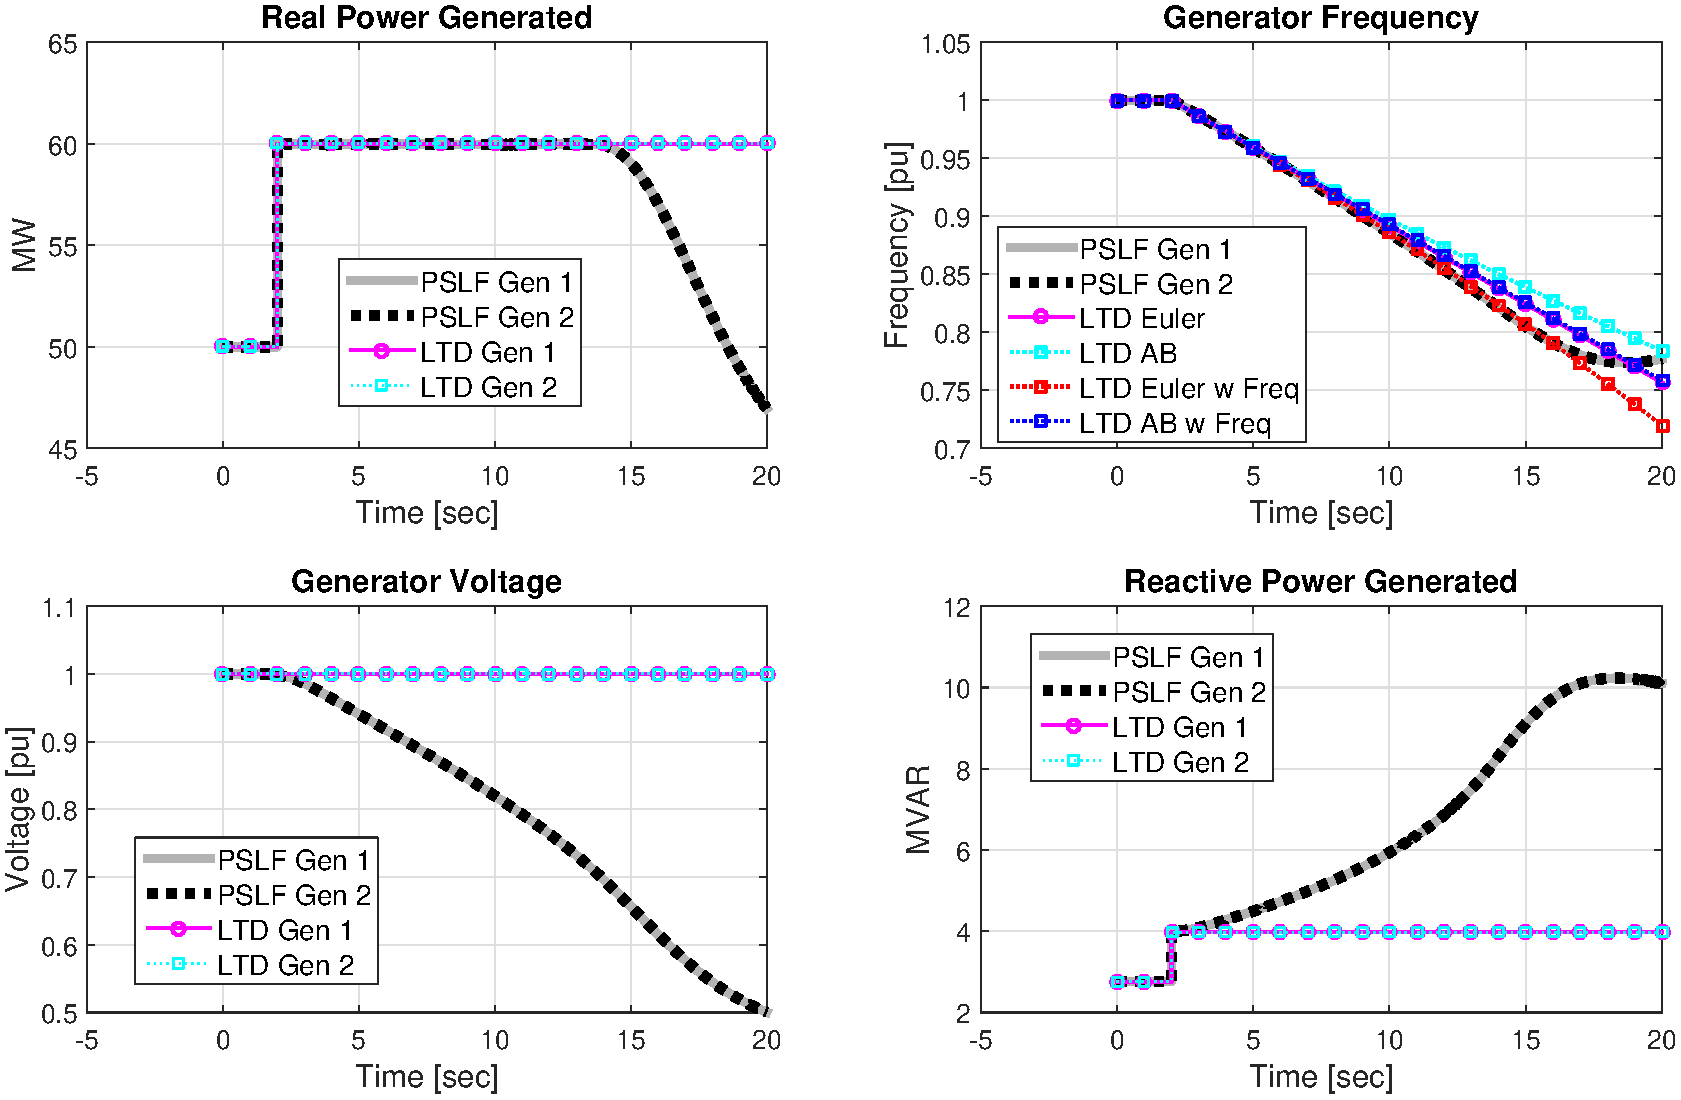
\includegraphics[width=\linewidth]{noGov_LTD01.pdf}
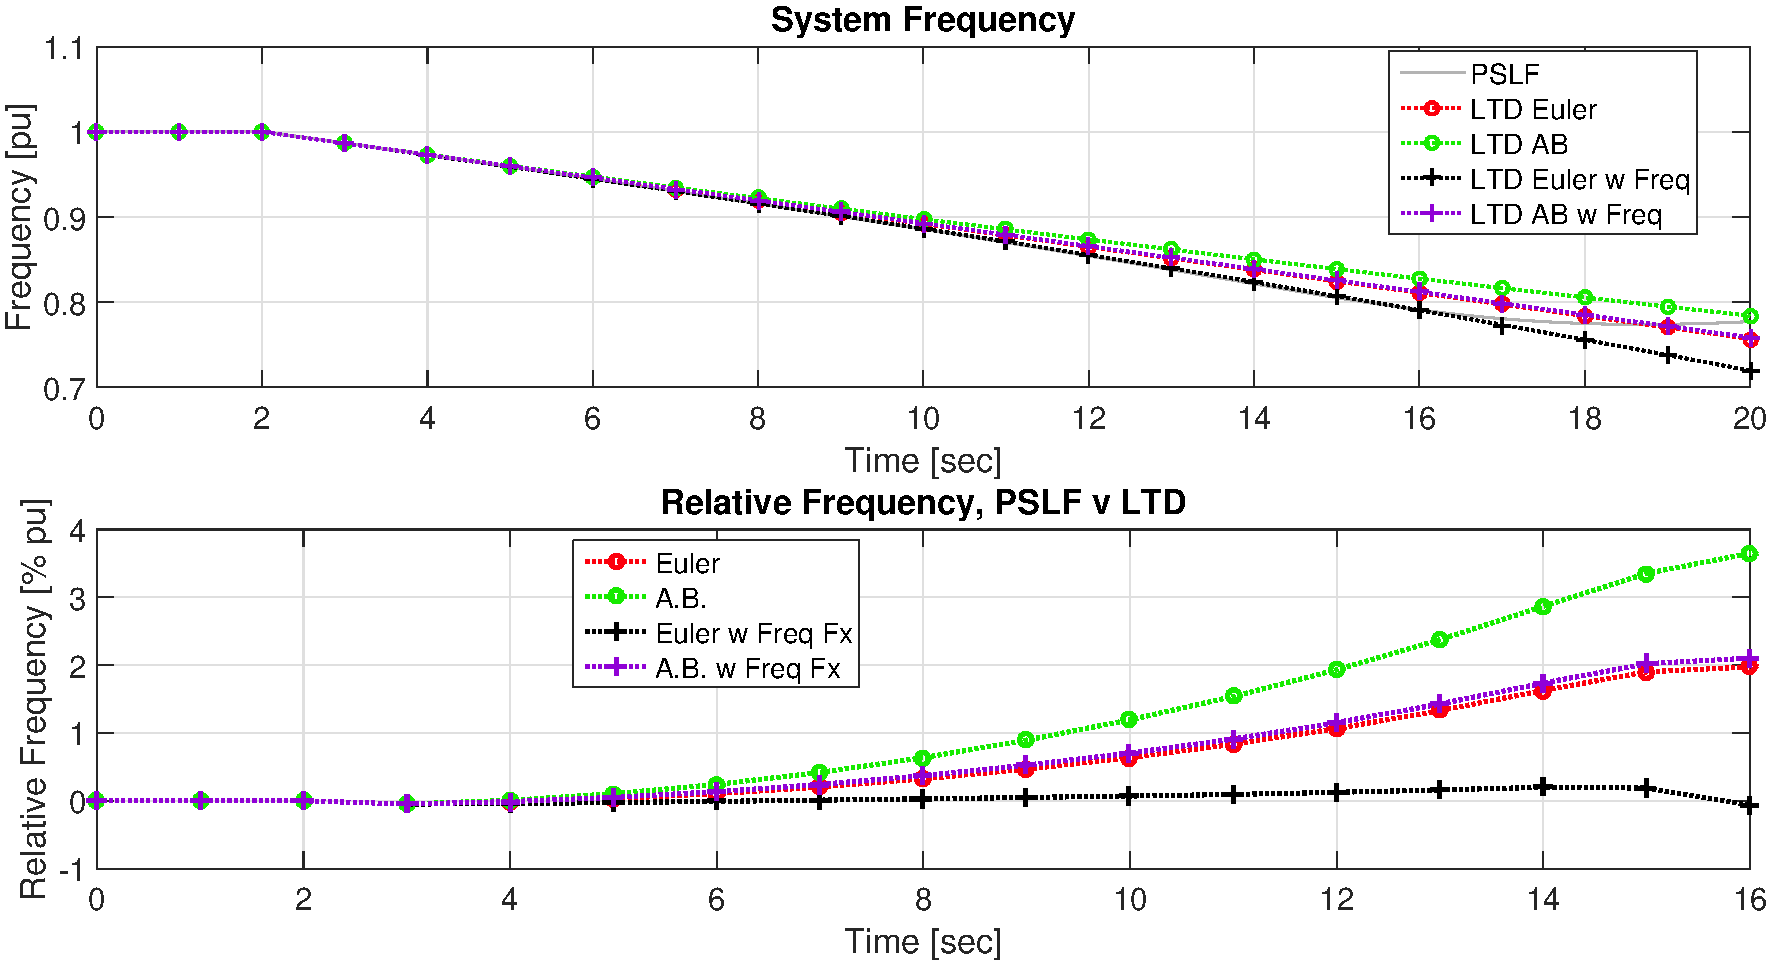
\includegraphics[width=\linewidth]{noGov_LTD04.pdf}

\end{document}